\documentclass[10pt,a4paper]{article}
\usepackage[utf8]{inputenc}
\usepackage[italian]{babel}
\usepackage{amsmath}
\usepackage{amsfonts}
\usepackage{amssymb}
\usepackage{float}
\usepackage{graphicx}
\graphicspath{{./images/}}
\usepackage{mathtools}
\usepackage[]{algorithm2e}
\DeclarePairedDelimiter\abs{\lvert}{\rvert}
\usepackage[left=3.00cm, right=3.00cm, top=3.00cm, bottom=3.00cm]{geometry}
\author{Del Prete Giovanni (1035205), Ghilardi Nicola (1040848), Polver Marco (1040386)}
\title{BookSales UniBG: iterazione 2}

\begin{document}
	
	\maketitle
	\tableofcontents
	
	\section{Algoritmo: il clustering}
	Il clustering è un algoritmo di apprendimento non supervisionato (machine learning) che ha l'obiettivo di ricercare gruppi di oggetti tali che  
	gli oggetti appartenenti a un gruppo siano “simili” tra loro e differenti dagli oggetti negli altri gruppi. Dunque, in statistica, è una tecnica di 
        analisi multivariata dei dati volta al raggruppamento di elementi omogenei in un insieme di dati.\\
        Oggi le tecniche di clustering sono diffuse in diversi campi applicativi, tra i quali: il marketing, l'analisi del territorio, le assicurazioni  gli studi sismici e l'image processing.  Uno degli usi più comuni che viene fatto dei cluster, in ambito economico, 
        è proprio la segmentazione di mercato, che può essere riferita a consumatori o a categorie di prodotti con lo scopo di valutare le caratteristiche e i comportamenti dei consumatori, personalizzando l’offerta
        e incrementando dunque la quantità di prodotti venduti.
              \begin{figure}[H]
		\centering
		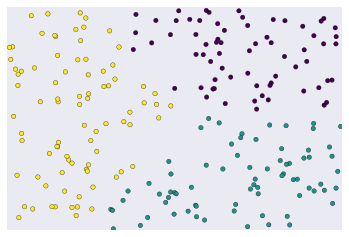
\includegraphics[scale=0.9]{Cluster.png}
		\caption{Cluster}
		\end{figure}
		\newpage        
        		\subsection{K-means clustering}
        		Il k-means clustering è l'algoritmo di clustering più utilizzato sia in ambito accademico che in ambito industriale e funziona nel seguente modo.
        		\begin{enumerate}
        		\item Scegliere il numero di k clusters in cui raggruppare il dataset.
        		\item Selezionare casualmente k centroidi iniziali (con centroide si intende il centro geometrico di ogni cluster).
        		\item Calcolare la distanza tra ogni centroide e tutte le osservazioni.
        		\item Assegnare ognuna delle osservazione al cluster rappresentato dal centroide più vicino.
        		\item Ricalcolare la posizione dei centroidi come la posizione media delle osservazioni appartenenti al cluster che il centroide rappresenta.
        		\item Ripetere dal punto 3, finchè nessuna osservazione cambierà più il proprio cluster di appartenenza.
        		\end{enumerate}
		\textbf{Problema}: come scegliere a priori il numero di clusters?\\
		La soluzione a questo problema sta nel testare in modo iterativo più valori di k e confrontarli. 
		Per valutare il risultato viene analizzata la funzione di costo:
		\[
		J(k)=\frac{1}{k}
		\sum_{i=1}^k
		\frac{1}{n}
		\sum_{j=1}^n
		\abs{p\textsubscript{j}-c\textsubscript{i}}
		\]
		Tale funzione di costo è la media delle distanze medie delle osservazioni dal centroide del proprio cluster. E' facile notare che aumentando il numero di
		cluster diminuirà, di conseguenza, la media delle distanze delle osservazioni dai centroidi; dunque la funzione di costo è decrescente.\\
		L'\textit{elbow method} è un metodo ''grafico'' che consente di determinare il numero di cluster ideale valutando la pendenza della funzione di costo.
		Come si evince dalla Figura 2, il valore ottimo di k è prossimo al punto dove la funzione di costo inizia a decrescere più lentamente.
		\begin{figure}[H]
		\centering
		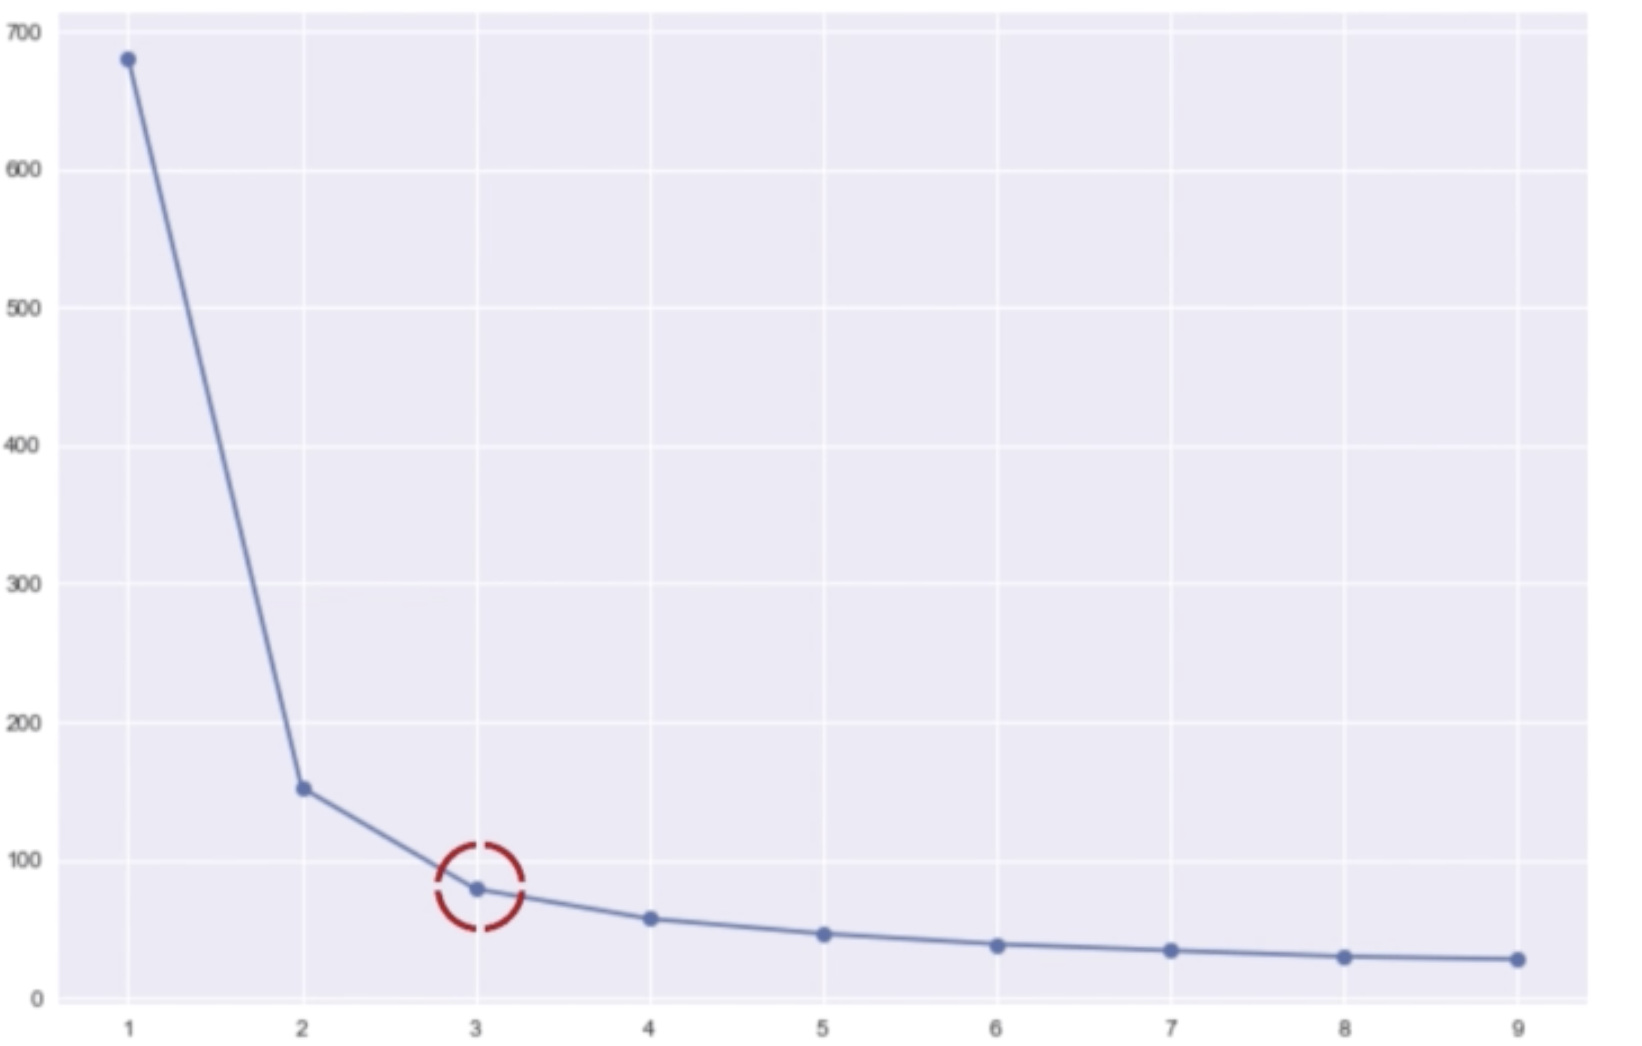
\includegraphics[scale=0.5]{elbow_method.png}
		\caption{Elbow method}
		\end{figure}
		
		Di seguito si può osservare in pseudocodice la funzione che assegna ad ogni osservazione un cluster di appartenenza.\\
		\\
		\begin{algorithm}[H]
		\KwData{Matrice delle osservazioni, k cluster}
		\KwResult{Cluster di appartenenza di ogni osservazione }
		creazione k centers casuali\;
		\While{centers non cambia}{
			distanza $\gets$ centers - osservazione\;
			\For{ogni cluster}{
				\If{distanza minima}{
					clusters $\gets$ osservazione\;
				}
			}
			centers $\gets$ media osservazioni clusters
		}
		\textbf{return} clusters
		\end{algorithm}
		
		La funzione di calcolo dei cluster è chiamata da una funzione che calcola, tramite l'elbow method, il numero ottimale di cluster in cui dividere le osservazioni. Essendo l'elbow method un 
		metodo di valutazione grafico, è stato necessario impostare sperimentalmente e compatibilmente con il problema, un valore target di derivata da raggiungere per ottenere il numero adeguato di cluster. 
		E' stato necessario impostare altri due parametri per limitare la complessità temporale del processo di clustering: una valore massimo di k\_{max} da testare e un contatore per limitare le iterazioni.  \\
		\\
		\begin{algorithm}[H]
		\KwData{media delle distanze medie delle osservazioni dal centroide per ogni cluster}
		\KwResult{numero k di cluster ottimale}
		k = 2\;
		fisso un k\_{max} di cluster\;
		\While{$\left|derivata\right|$ $<$  0.1 e  k $<$ k\_{max} e count $<$100}{
			calcolo cluster e centroidi\; 
			cluster\_{cost} $\gets$ media delle distanze dal proprio centro di un cluster\;
			total\_{cost} $\gets$ media di cluster\_{cost}\;
			derivata $\gets$ $total\_{cost}_{k-1} - total\_{cost}_{k}$\;
			k $\gets$ k + 1\;
			count $\gets$ count + 1\;
		}
		\textbf{return} k
		\end{algorithm}
		
		\subsection{Il clustering in BookSales Unibg}
		L'algoritmo di k-means clustering è stato utilizzato in BookSales Unibg con l'obiettivo di suddividere in cluster gli utenti sulle basi dei loro interessi.
		L'algoritmo assegna ad ogni studente un cluster di appartenenza basandosi sui titoli presenti nella sua Wish List e Interesting Title. Ogni libro 
		presente in BookSales Unibg appartiene ad una categoria: le features di ogni studente sono il numero di libri che interessano allo studente 
		appartenenti ad ogni categoria.
		Le categorie in cui sono stati suddivisi i libri sono:
		\begin{itemize}
			\item Fisica
			\item Matematica
			\item Informatica
			\item Meccanica
			\item Elettronica
			\item Economia
			\item Automazione
		\end{itemize}
		L'algoritmo viene eseguito dall'applicazione automaticamente una volta al giorno.
		Dopo i risultati del clustering, ogni studente vedrà nella pagina Suggested Adds i titoli in linea con i propri interessi.\\
		Dato il numero elevato di features e di cluster non è possibile visualizzare graficamente i risultati di un'esecuzione dell'algoritmo.

\section{Funzionalità aggiunte}
All'applicazione sono state aggiunte funzionalità per renderla più user friendly. La prima è quella di fornire un'anteprima della copertina dei libri in copertina. Le immagini vengono caricate nel database e in fase di ricerca vengono lette e caricate nella schermata.\\
Ogni utente inoltre ha la possibilità di aggiungere un libro nella propria wishlist. Per permettere tale operazione si è aggiunto un tasto \textit{Add to wishlist}.

\section{Resoconto test}
Con il fine di verificare la corretta implementazione delle nuove funzionalità e di garantire la correttezza delle funzionalità aggiunte in precedenza, è stato creato un nuovo caso di test con Selenium WebDriver per coprire il caso d'uso UC4 (Aggiunta di in un annuncio in "wishlist") ed è stata eseguite l'intera sequenza di test.\\
Il risultato ottenuto è stato quello atteso, ovvero tutti i test hanno dato risultato positivo.
\begin{figure}[H]
	\centering
	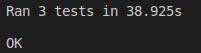
\includegraphics[scale=0.9]{tests_i3b.png}
	\caption{Risultato dei test}
\end{figure}
\end{document}